
In the previous sections we considered the gravity field of a given
mass distribution.
For self-gravitating planets of sufficient size {\bf the local
density depends on the pressure, through selfcompression} i.e.
the compression of the material caused by the planets own gravity field.
As we have seen in previous sections the lithostatic pressure
depends on the gravity field and the density distribution. 
It follows that the determination of the density, gravity and
pressure are coupled problems that must be solved simultaneously
and can not be solved separately.
Here we will consider the solution of such coupled problems.

From observations of the average density of surface rocks of some
$2.7 \cdot 10^3~\mathrm{kg/m^3}$ 
and the known mean density of the Earth 
$5.5 \cdot 10^3~\mathrm{kg/m^3}$, 
it follows that the surface density is less than half the 
mean Earth value.
{\bf The difference between both density values suggests a density increase
in the interior which could be related either to different composition at depth}, 
for example corresponding to a dense metallic core, 
{\bf and/or the effect of selfcompression in an otherwise 
homogeneous planet}. 
Solid state phase transitions of mantle material due to increasing pressure
can also explain part of the high mean density value.

From the nineteenth century on, models of the internal density 
distribution of the earth have been investigated. 
These models have in common that the radial density distribution is 
parameterized in a simple way with a small number of parameters,
typically two, which are then adjusted to the known data such as 
the surface density and the Earth's total mass or moment of inertia.

%An early example of this approach is the parameterization of Laplace,
%\begin{equation}
%   \rho(r) = \rho_0 \frac{\sin(qr)}{qr}
%\label{laplace_rho}
%\end{equation}
%where $\rho_0$, the density at the centre, and the parameter $q$ 
%can be expressed in the surface density $\rho_0$
%and the total mass $M$.

%Besides the planetary mass and surface density, models
%for the interior density distribution
%are also constrained by the planets moment of inertia $I$
%(\ref{mominert_uniform_sphere})
%that can be determined from (satelite) geodetic and astronomical
%observations.
%For Earth the following values for the total mass and moment of inertia
%prefactor have been found,
%\begin{equation}
%M = 5.97 \cdot 10 ^{24}~\mathrm{kg},~
%I = 0.3307 M R^2 
%\end{equation}
%where $R = 6371$ km is the mean radius.
%The observed moment of inertia prefactor $f=0.3307$ is smaller than the 
%value $0.4$ for a homogeneous sphere (see \ref{sect_scalarmomint}), 
%another indication of mass concentration towards the earth's centre.

In the following the relation between density, gravity and pressure in
a self-gravitating planet will be investigated in a more
self consistent way.

~\\
For a spherically symmetric density distribution the corresponding magnitude of the 
gravity acceleration vector is given by (\ref{eqn_g_rad_comp}),
\begin{equation}
g(r) = |{\bm g}({\bm r})|=|g_r(r)| = \frac{4 \pi G}{r^2}
       \int_0^r \rho(r^{'}) r^{'2} dr^{'}
     = \frac{Gm(r)}{r^2}
\label{g_accel}
\end{equation}
where $m(r)$ is the mass of a sphere of radius $r$ and $\rho(r)$
is the corresponding radial density profile.

\vspace{0.5cm}

\fbox{
\begin{minipage}{0.9\textwidth}
\begin{problem}
{\small \it
Use (\ref{g_accel}) to show that it is not possible to derive a {\it unique}
radial mass distribution of a spherically symmetric planet from
the observed surface value of the gravity field alone.
This can be verified by showing that multiple density profiles exist that
produce the same surface gravity. 
To illustrate this 
sketch a schematic internal radial profile of the
gravity acceleration in a comparison of two spherically symmetric
planets of identical mass $M$ and radius $R$.
The first one is a homogeneous planet with density $\rho_0$
and the second one is a differentiated planet with a uniform high 
density core $\rho_c=\rho_0+\delta \rho$ and less dense mantle 
$\rho_m=\rho_0-\delta \rho$.
Verify that these assumptions correspond to this special case
with volume fraction of the core $\phi_c =1/2$.

%The same external gravity field is obtained with a spherical
%shell of zero thickness and radius $r$, 
%with a uniform surface mass density $\sigma(r) = M/(4\pi r^2)$, 
%(a uniform mass sheet)
%as a special case of (\ref{def_equiv_mass}).
%It can be shown more generally that for the external gravity field
%of a non-spherically symmetric mass distribution, 
%equivalent non-uniform mass sheets
%can be defined generating the same external gravity field.

}
\end{problem}
\end{minipage}
}


\vspace{0.5cm}


From the above results the lithostatic pressure distribution can be 
obtained by substitution for the gravity acceleration and 
integrating the pressure gradient $dP/dr = - \rho g$.
Assuming a zero pressure value at the surface this results in,
\begin{equation}
P(r) = \int_r^R \rho(r^{'}) g(r^{'}) dr^{'}
     = 4 \pi G \int_r^R \rho(r^{'}) 
                 \left \{
                      \frac{1}{r^{'2}}
                      \int_0^{r^{'}}
                           \rho(r^{''}) r^{''2} dr^{''}
                 \right \}
               dr^{'}
\label{pressure_integral}
\end{equation}


The pressure in the Earth's interior reaches values over 350 GPa
as shown in Fig. \ref{Fig_PREM}.
For such high pressure values the effect of self-compression 
on the density is significant.
In the following this effect is further explored.

%--------------------------------
\paragraph{The bulkmodulus}

  An isotropic linear elastic solid can be described by two 
  independent elasticity parameters, for instance the Lam\'{e} parameters
  $\lambda$ and $\mu$ \footnote{https://en.wikipedia.org/wiki/Elastic\_modulus}.
  The bulkmodulus can be expressed in the Lam\'{e} parameters as,
  $K = \lambda + \frac{2}{3}\mu$.
  The bulkmodulus $K$ and the shearmodulus $\mu$ are 
  the most commonly used parameters to specify the 
  elastic parameters of Earth materials.

The bulk modulus $K$ 
of a substance measures the substance's resistance to uniform compression. 
It is defined as the ratio of the infinitesimal pressure increase to the 
resulting relative decrease of the volume. Its SI unit is the Pascal, 
and its dimensional form is $M^1L^{-1}T^{-2}$.

\begin{center}
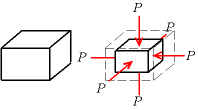
\includegraphics[width=6cm]{images/gravity/bulkmodulus}
\end{center}


The incompressibility $K$, or bulkmodulus
, is defined as,
\begin{equation}
   \frac{1}{K} = \frac{1}{\rho} \frac{d\rho}{dP}
\label{def_incompres}
\end{equation}
By substitution of $dP = - \rho g dr$ in (\ref{def_incompres}) 
we derive a differential equation for the density profile
of a compressible planet model,
\begin{equation}
  \frac{1}{K} = \frac{-1}{\rho^2 g} \frac{d\rho}{dr}
    \Rightarrow 
  \frac{d\rho}{dr} = - \frac{\rho^2 g}{K}
%  \frac{1}{\rho} \frac{d\rho}{dP}
%    =
%   \frac{1}{\rho} \frac{d\rho}{dr}\frac{dr}{dP} =
%   \frac{1}{K} 
%   ~\rightarrow 
%    \frac{d\rho}{dr} 
%       = \left ( \frac{dr}{dP} \right )^{-1} \frac{\rho}{K} 
%       = - \frac{\rho^2 g}{K} 
\label{dens_ode}
\end{equation}

%--------------------------------
\paragraph{Parameterization of the bulkmodulus}
The radial density distribution for a selfcompressing planet can be 
obtained from (\ref{dens_ode}) once the bulkmodulus $K$ is known.
We will first consider simple cases where $K$ is either a uniform
constant or it is parameterized in terms of the density.

\vspace{0.5cm}
\fbox{
\begin{minipage}{0.9\textwidth}
\begin{problem}
\label{problem_singular-density-model}
{\small \it
  Assume both $K$ and $g$ in (\ref{dens_ode}) 
  to be uniform in the mantle and derive the
  following density profile,

%\footnote{
%  Hint:
%  First order ordinary differential equations like 
%  (\ref{dens_ode}) are of so called separable form, 
%  \begin{equation}
%   \frac{dy}{dx} = P(y)Q(x)
%  \end{equation}
%  (see for instance, E.L. Ince, 
%   {\it Integration of ordinary differential equations}, 
%   Oliver and Boyd, 1956)
%  in which case they can be integrated in the following way,
%  \begin{equation}
%   \frac{dy}{P(y)} = Q(x) dx
%    \rightarrow
%   \int \frac{dy}{P(y)} = \int Q(x) dx + C
%    \rightarrow
%  \end{equation}
%   In cases where the lefthand integral is a known function, say $f(y)$,
%   the solution is obtained by the inverse function,
%  \begin{equation}
%    y(x) = f^{-1}
%            \left ( \int Q(x)dx + C \right )
%  \end{equation}
%  Example: $dy/dx= - y^2 e^{-x}~,~~x\ge 0$, 
%  \begin{equation}
%    \int -\frac{dy}{y^2} = \int e^{-x} dx + C
%    \rightarrow
%     \frac{1}{y} = -e^{-x}+ C
%    \rightarrow
%     y(x) = \frac{1}{C -e^{-x}}
%  \end{equation}
%  The integration constant $C$ can be expressed in an
%  initial condition, $C=1+1/y(0)$.
%}
  \begin{equation}
     \rho(z) = \frac{\rho_0}{1-\frac{\rho_0 gz}{K}}
  \label{eqn_singular-density-model}
  \end{equation}
  where $z=R-r$ is the depth coordinate and
  $\rho_0=\rho(0)$ is the surface density value.

  \begin{itemize}
  \item
  Compute the depth $z_1$ where the expression (\ref{eqn_singular-density-model}) 
  becomes singular,
  i.e. $\rho \rightarrow \infty$, suggesting infinite compression of the material.
  To do this assume Earth(mantle)-like values of the incompressibility,
   $K=400 \mathrm{GPa}$ (see Fig.\ref{Fig_pressure_incompress}) 
  and the surface density $\rho_0 = 3 \cdot 10^3~ \mathrm{kg/m^3}$.
  \item
  Now consider a simplified model of a large rocky exoplanet of Earth-like
  composition with $M=8 M_{\oplus}$ and $R=1.5 R_{\oplus}$.
  Assume uniform gravity (adapted for the given $M,R$) and uniform 
  incompressibility $K$.
  Do you now find the singular depth $z_1$ within the depth range of the planet?
  Comment on the assumption of a uniform gravity field in view of the models
  presented in section \ref{sect_param_densmod}. 
  \end{itemize}
}
\end{problem}
\end{minipage}
}



\vspace{0.5cm}

\fbox{
\begin{minipage}{0.9\textwidth}
\begin{problem}
{\small \it
The result of problem \ref{problem_singular-density-model}
gives the density depth distribution for the model with constant properties.
The resulting expression  (\ref{eqn_singular-density-model}) also contains
the uniform gravity acceleration.
A more fundamental relation between density and pressure,
not including gravity, can be derived 
for this model with constant material property $K$ as an equation of state (EOS)
for the density. 

Derive from the definition of the bulkmodulus (\ref{def_incompres}) 
the following logarithmic EOS for the density in terms of the 
static pressure,
%\footnote{
%Hint: evaluate the integral expression for pressure
%$P(z) = \int_0^z \rho g dz^{'}$ by substitution of 
%(\ref{eqn_singular-density-model}).
%}
\begin{equation}
 P = \ln \left ( \left ( \frac{\rho}{\rho_0} \right )^K \right )
\label{logarithmic-EOS}
\end{equation}
Show that the above EOS (\ref{logarithmic-EOS}) can be inverted to obtain an explicit expression
for density as a function of pressure. 
%\begin{equation}
% \rho(P) = \rho_0 \exp \left ( \frac{P}{K} \right )
%\label{exponential-density}
%\end{equation}
}
\end{problem}
\end{minipage}
}

\vspace{0.5cm}

The singular behavior in the density model of problem 
\ref{problem_singular-density-model} is a result
of the assumed uniform $g$ and $K$ in (\ref{dens_ode}).
While $g$ is reasonably constant with depth in the mantle,
as illustrated in Fig. \ref{Fig_PREM},
$K$ is not.
The incompressibility increases with increasing depth/pressure
and as a result
the compression remains  finite for earth-like conditions.
The incompressibility can be expressed in the density and the 
seismic wave velocities,
$v_p = \sqrt{(\lambda + 2\mu)/\rho}$,
$v_s = \sqrt{\mu/\rho}$. 
With $K=\lambda + \frac{2}{3} \mu$ this becomes $K= \rho ( v_p^2 - 4/3 v_s^2)$. 
A radial profile $K(P(r))$ can therefore be derived, from the seismic velocities 
determined from inversion of traveltime
tables of longitudinal and shearwave seismic arrivals. 

The $K(P(r))$ profile derived from the PREM model of 
Dziewonski and Anderson (1981) appears to be roughly linear as shown
in the following figure: 

\begin{center}
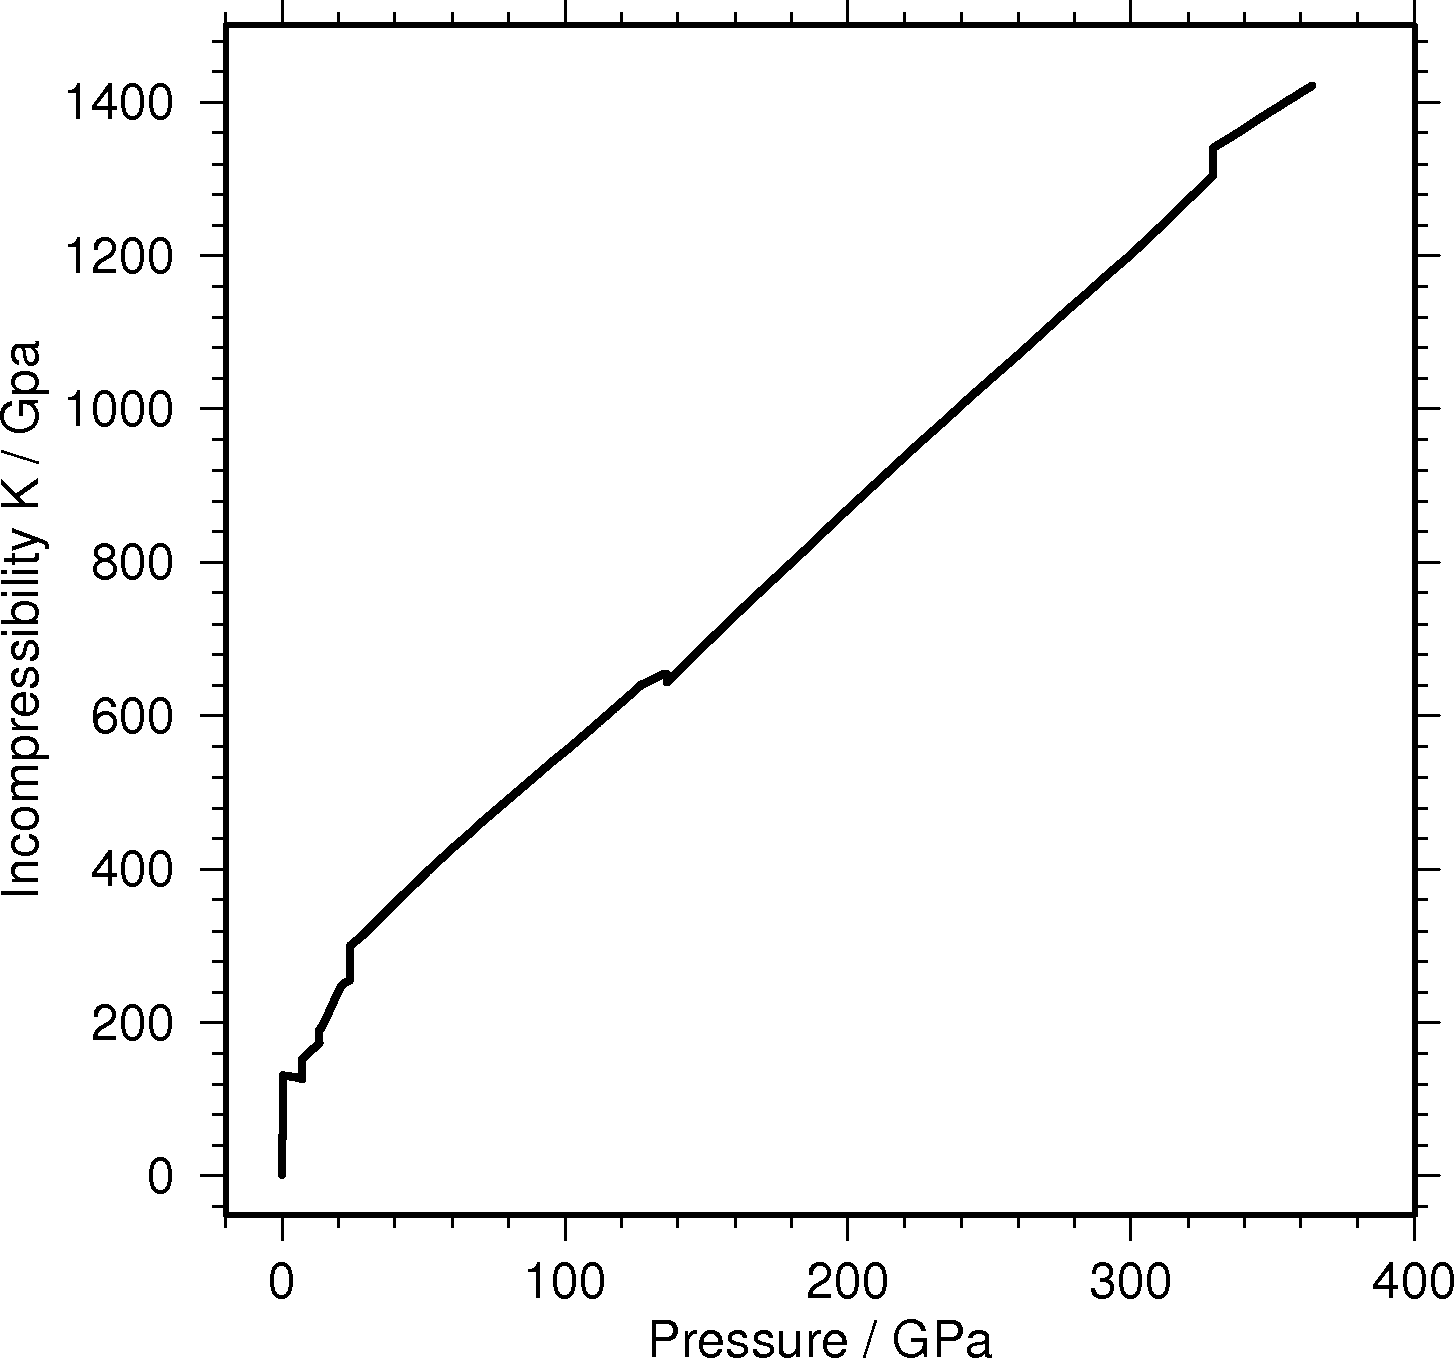
\includegraphics[width=6cm]{images/gravity/pressure_incompress}\\
{\captionfont Incompressibility profile derived from the PREM model.}
\end{center}

A linear relation between bulkmodulus and pressure as suggested
by this figure is also obtained
using the following
power law parameterization for the bulkmodulus in terms of the
density $K(\rho)$.
\begin{equation}
K = C \rho^n
~~ \Rightarrow
\ln(K) = \ln(C) + n\ln(\rho) 
~~ \Rightarrow
n = \frac{d \ln (K)}{d \ln (\rho)} =  \frac{dK}{dP} = K_0^{'}
\label{K-rho}
\end{equation}
where $C$ is a constant.
The constant pressure derivative in this model 
implies a linear pressure relation $K(P)=K_0 + K_0^{'}P$.
This appears to approximate the distribution of $K$ in particular in the
lower mantle as determined from seismological data in the PREM model. 
$K_0^{'} \approx 4$ for the magnesium-iron sillicates 
$\mathrm{(Mg,Fe)SiO_3}$ (perovskite)
and dense oxides $\mathrm{(Mg,Fe)O}$ (w\"{u}stite),
representative for 
the earth's deep mantle.

\paragraph{The Murnaghan e.o.s.} 
An equation of state directly relating the density or specific volume,
$V = 1/\rho$,
to pressure can be derived from such an 
`ansatz' of a linear pressure dependence $K = K_0 + K_0' P$
as shown in the following,
\begin{equation}
 \frac{1}{\rho} \frac{d\rho}{dP} =\frac{1}{K}
 ~\rightarrow~
 \frac{1}{V} \frac{dV}{dP} =-\frac{1}{K}
 ~\rightarrow~
  dP = -(K_0+K_0'P)\frac{1}{V} dV
\end{equation}
\begin{equation}
  \int_0^P \frac{dP'}{K_0+K_0'P'}
   =
 -\int_{V_0}^V \frac{1}{V'}dV'
   =
  \int_V^{V_0} \frac{1}{V'}dV'
   =
  \ln \left ( \frac{V_0}{V} \right )
\end{equation}
Substitution in the integral over pressure of 
$K_0+K_0'P'=x$, $dx=K_0'dP'$ gives,
\begin{equation}
 \int_{x_0=K_0}^{x_P=K_0+K_0'P}
  \frac{1}{K_0'} \frac{dx}{x}
  =
  \frac{1}{K_0'} \ln \left ( \frac{K_0+K_0'P}{K_0} \right )
  =
  \ln \left ( \frac{V_0}{V} \right )
\end{equation}
\begin{equation}
  1 + \frac{K_0'P}{K_0}
  =
  \left ( \frac{V_0}{V} \right )^{K_0'}
  ~\rightarrow~
  P = \frac{K_0}{K_0'} 
      \left (
        \left (
            \frac{V_0}{V}
       \right )^{K_0'}  -1
     \right )
\label{eqn_murnaghan_eos}
\end{equation}
This relation is known as the Murnaghan equation of state (EOS).

The Murnaghan equation of state is a relationship between the volume of a body and the pressure to which it is subjected. 
This is one of many state equations that have been used in earth sciences and shock physics to model the behavior 
of matter under conditions of high pressure. It owes its name to Francis D. Murnaghan 
who proposed it in 1944 to reflect material behavior under a pressure range as wide as possible 
to reflect an experimentally established fact: {\bf the more a solid is compressed, the more difficult it is to compress further}.

The Murnaghan equation is derived, under certain assumptions, from the equations of continuum mechanics. 
It involves two adjustable parameters: the modulus of incompressibility $K_0$ and its first derivative 
with respect to the pressure, $K_0'$, both measured at ambient pressure. 
In general, these coefficients are determined by a regression on experimentally obtained values 
of volume $V$ as a function of the pressure $P$. 
These experimental data can be obtained by X-ray diffraction or by shock tests. 
Regression can also be performed on the values of the energy as a function of the volume obtained from ab-initio and molecular dynamics calculations.


%~\\
%Substitution in (\ref{secorder-ode}) results in
%Emden's equation,
%\begin{equation}
%\frac{d}{dr} \left (
%                     r^2 \rho^{n-2} \frac{d\rho}{dr}
%            \right )
%=
%   - \frac{4 \pi G}{C} r^2 \rho = - A^2 r^2 \rho
%\label{emden_eqn}
%\end{equation}
%This model leads to a non-linear differential equation for the density 
%profile $\rho (r)$, which can be solved numerically.
%For the special case $n=2$ the equation is linear and can be solved
%analytically (see below).
%
%\begin{problem}
%Show that a related parameterization by Laplace, 
%$dP/d\rho = C \rho$, leads to (\ref{K-rho}) with $n=2$,
%(Poirier, Introduction to the physics of the Earth's interior, 2000).
%Show that the corresponding density is,
%\begin{equation}
% \rho(r) = \rho(0) \sin ( Ar) /Ar
%\label{eqn_laplace_n2}
%\end{equation}
%{\it Hint:} substitute  $\rho(r) = \Psi(r) /r$ and solve the integration
%constants from the radial symmetry, $d\rho/dr=0$, and prescribed density 
%$\rho (0)$ at $r=0$.
%\end{problem}
%
%\begin{problem}
%The above model is used as an approximation for giant gas planets like 
%Jupiter.
%The planet outer radius is then defined by the zero density value.
%Verify that in this way the planetary radius is fixed and in particular,
%independent of the total mass of the planet.
%Give a physical interpretation of this characteristic.
%\end{problem}



\vspace{0.5cm}
\fbox{
\begin{minipage}{0.9\textwidth}
\begin{problem}
 {\small \it
  Derive an explicit expression for the pressure dependent density
  from the Murnaghan equation of state (\ref{eqn_murnaghan_eos}).
\newline
  Answer:
  \begin{equation}
     \rho(P) = \rho_0 \left (
                              \frac{K_0^{'}P}{K_0} + 1
                     \right )^{1/K_0^{'}}
  \end{equation}
 }
\end{problem}
\end{minipage}
}


\vspace{0.5cm}
\fbox{
\begin{minipage}{0.9\textwidth}
\begin{problem}
\label{problem_powerlaw-K_constant-g}
 {\small \it
  In problem \ref{problem_singular-density-model} 
  we have seen that a simple model with uniform 
  incompressibility and gravity
  $K=K_0$ and $g=g_0$ leads to physically impossible solutions.
  In a refined version of this model, applied to the Earth's mantle,
  $g=g_0$ is maintained (compare Fig.\ref{Fig_PREM}), 
  and $K$ is parameterized using the powerlaw relation (\ref{K-rho}).
  \newline
  Derive the following density profile for the model corresponding to 
  (\ref{K-rho}).  
  \begin{equation}
     \rho(r) = \rho_0 
        \left (
              1 + (n-1) \frac{\rho_0 g_0 z}{K_0}
       \right )^{\frac{1}{n-1}}
  \label{eqn_g0_n2}
  \end{equation}
  where $z=R-r$ is the depth coordinate and the 0 subscript refers to
  zero pressure conditions. 
  Note that 
  the singularity for $\rho_0 g_0 z / K_0 =1$ 
  in problem \ref{problem_singular-density-model} is absent in this model.
 }
\end{problem}
\end{minipage}
}

\vspace{0.5cm}


A more widely used and more accurate EOS 
for a higher pressure range is the equation
derived by Birch (1952) from a consideration of 
elastic strain energy, known as the 
Birch-Murnaghan EOS (Poirier, 2000).

In other cases than the special simplified cases discussed above, 
in particular in problems \ref{problem_singular-density-model} and 
\ref{problem_powerlaw-K_constant-g},
the gravity acceleration varies also with depth.
Also more accurate equations of state may be necessary for very high pressure,
encountered in the deep interior of large (exo)planets,
that result in large compression.
Such models can be formulated in a more general way by the following coupled set
of equations for pressure, gravity and density.
\begin{equation}
  \frac{dP}{dr} = - \rho g
\label{mod_pressure_gradient}
\end{equation}
\begin{equation}
  g(r) = \frac{G m(r)}{r^2} 
\label{mod_gravity_accel}
\end{equation}
\begin{equation}
  F(\rho,P,T) = 0
\label{mod_EOS}
\end{equation}
where the radial mass distribution $m(r)$ is defined as in (\ref{def_equiv_mass}).
A model based on 
(\ref{mod_pressure_gradient}),
(\ref{mod_gravity_accel}), and 
(\ref{mod_EOS}) 
can be constructed for the internal structure 
(density, gravity, pressure) of a planet of given mass $M$ and composition,
i.e. with given parameters of the EOS (\ref{mod_EOS}) such as 
$\rho_0, K_0, K_0'$ in the Murnaghan EOS (\ref{eqn_murnaghan_eos}). 
Consider the application of such a model to a planet for which only the 
planet mass $M$ is known.
\footnote{
Such models can be applied to exoplanets that are recently being discovered
https://en.wikipedia.org/wiki/Methods\_of\_detecting\_exoplanets .
For some of these planets, detected from radial velocity variations of the star,
only the planet mass $M$ is known.
}
Assume a homogeneous terrestrial (rocky) planet without a distinct metallic core. 
Assuming an earth-mantle like composition, representative values of the
EOS parameters can be used, to solve the coupled model equations in 
the following iterative scheme.
\begin{enumerate}
  \item
  Define a grid along the radial coordinate 
  $r_i, i=1,\ldots, N,~ r_1=0$. 
  This grid defines a subdivision of the interior in $N-1$ concentric layers and
  must be chosen large enough, i.e. $r_N > R$.
  \item
  Choose an initial estimate of the central pressure $P^{(1)}(0)$.
  \item
  \label{cycle_layer_loop}
  In a loop over the internal layers, starting upward from the centre,  
  first compute the pressure decrement over the layer from (\ref{mod_pressure_gradient}).
  This is then used to obtain the pressure at the next grid point and
  corresponding density from the EOS (\ref{mod_EOS}).
  From the computed density the corresponding mass distribution $m(r_i)$ and
  gravity $g(r_i)$ (\ref{mod_gravity_accel}) follow.
  \item
  \label{item_pressure-correction}
  The layer iteration in the previous item is stopped when a zero pressure 
  value has been reached. The radial level reached this way now defines 
  the next approximation of the planetary radius $R^{(j)}$ and 
  $M^{(j)}=m(R^{(j)})$ is a new approximation of the planet mass $M$.
  \item
  From the total mass defect $\Delta M^{(j)} = M^{(j)} -M$ a correction 
  to the central pressure is computed as $\Delta P^{(j)}$,
  (problem \ref{problem_pressure-correction}). 
  In the next iteration the radial integration is repeated from item 
  \ref{cycle_layer_loop} 
  with an updated central pressure $P^{(j+1)}(0) = P^{(j)}(0) + \Delta P^{(j)}$
  and this iterative procedure is repeated until convergence is reached, 
  i.e. until $|\Delta M^{(j)}|/M$ drops below a specified tolerance value. 
\end{enumerate}





\fbox{
\begin{minipage}{0.9\textwidth}
\begin{problem}
 \label{problem_pressure-correction}
 {\small \it
 A correction for the central pressure in item \ref{item_pressure-correction} 
 can be estimated by distributing the mass defect $\Delta M^{(j)}$ 
 over a spherical shell of thickness $\Delta R^{(j)}$, positioned at the surface,
 and computing an approximate pressure $\Delta P^{(j)}$ at the bottom of this shell.
 
 Derive the following expression for the thickness of this spherical shell,
 \begin{equation} 
  \frac{\Delta R^{(j)}}{R^{(j)}} = 
  \left ( \frac{\Delta M^{(j)}}{M^{*(j)}} + 1 \right )^{1/3} -1
 \end{equation} 
 Where $M^{*(j)} = \frac{4\pi}{3} \rho(R^{(j)}) {R^{(j)}}^3$.

The correction for the central pressure is then defined as,
$\Delta P^{(j)} = \rho(R^{(j)}) g(R^{(j)}) \Delta R^{(j)}$.

 }
\end{problem}
\end{minipage}
}

\vspace{0.5cm}



%Now consider a two-layer model consisting of a dense metallic core and silicate mantle.
%How could the above schematic solution be adapted for such a two-layer model if the 
%mass fraction $X_c = M_c/M$ is known? What other information will you need to do an
%actual model calculation?
